\chapter{\textit{Document Planning}}
\label{cap:document_planning}

En la arquitectura presentada en el capítulo~\ref{cap:nlg_intro} mencionamos que el \emph{document planner} es el responsable de decidir que información comunicar (determinación de contenido) y como deberá estar estructurada esta información en el texto final (estructuración de documento). El \textit{document planner} será el encargado de que el documento final contenga toda la información requerida por el usuario y de que la misma se encuentre estructurada de una forma razonablemente coherente. El resultado de esta etapa será un \emph{document plan} en el cual se especificará qué contenido debe ser incluido en el texto final y de que forma deberá estar estructurado.


A continuación detallaremos las tareas que debe realizar el \textit{document planner}, describiremos brevemente la entrada y salida del mismo, definiremos como modelar los elementos informativos (pertenecientes a nuestro \emph{document plan}) y finalmente estudiaremos la estructuración del documento.

\section{Tareas del \textit{document planner}}
Como mencionamos anteriormente, el \textit{document planner} será el encargado de llevar a cabo las tareas de: \emph{determinación de contenido} y \emph{estructuración de documento}. A continuación describiremos brevemente cada una de estas tres tareas.

La \emph{determinación del contenido} es el nombre que se le da a la tarea de decidir y obtener la información que debemos comunicar en un texto. Este proceso generalmente involucra uno o más procesos de \emph{selección}, \emph{resumen} y \emph{razonamiento con los datos} de entrada.

%TODO ejemplos?
\bigskip
\noindent
\textbf{Selección:} es el proceso encargado de recopilar un subconjunto de la información de entrada para luego poder ser comunicada al lector. El objetivo de éste será proveerle al usuario la información relevante requerida por el mismo.

\bigskip
\noindent
\textbf{Resumen:} es necesario cuando los datos de entrada son muy granulados para ser comunicados directamente o si la información relevante consiste alguna generalización o abstracción de los mismos.

\bigskip
\noindent
\textbf{Razonamiento con los datos:} resulta un caso general de las dos anteriores, generalmente mas sofisticado y más específico del dominio de aplicación. 

\bigskip
Para nuestro sistema de NLG será necesario realizar una tarea de \emph{selección} que recopile el conjunto de clases de prueba que debemos describir. Luego veremos que procesando el resultado de la selección será posible obtener mejores descripciones. En particular llevaremos a cabo dos tareas del tipo procesamiento con los datos: \emph{eliminación de tautologías} y \emph{reducción de expresiones}. La primera nos permitirá filtrar expresiones que no añaden información adicional a la descripción final. Por otro lado, la \emph{eliminación de tautologías} será la encargada de simplificar algunas expresiones presentes en las clases de prueba. Llevar a cabo estas últimas dos tareas nos permitirá obtener descripciones mas concisas y claras. Ambas dos resultan consecuencia de la herramienta utilizada en nuestro trabajo para generar los casos de prueba (Fastest), es por esto que creemos importante realizarlas lo antes posible dentro del \textit{pipeline} de nuestro sistema para evitar dependencias entre etapas posteriores y la herramienta utilizada. En la sección \ref{cap:determinacion_contenido} retomaremos la \emph{determinación de contenido} donde estudiaremos mas en detalle las tareas mencionadas.

Por otro lado, una vez seleccionada y procesada la información que debemos comunicar, será la tarea de \emph{estructuración de documento} la encargada de agrupar dicha información con el fin de que el texto que debemos generar resulte coherente y posea una estructura que le permita al lector interpretar con facilidad el contenido del mismo. Necesitaremos considerar como organizar y estructurar la información que debemos transmitir en el texto final con el fin de producir una descripción razonablemente fácil de leer y comprender. La \emph{estructuración de documento} deberá encargarse de aspectos estructurales a nivel del documento que deseamos producir, donde se contemplarán, por ejemplo, cuestiones como el orden en el que debe que ser comunicada la información, como estará agrupada la misma, etc. El resultado de la \emph{estructuración de documento} (y del \textit{document planner}), será una estructura intermedia de nuestro \textit{pipeline} con la información antes mencionada a la que llamaremos \emph{document plan}. 

En las próximas secciones definiremos detalladamente la entrada y salida del \textit{document planner} estudiando cuales son los elementos informativos del \emph{document plan} y como los modelaremos, luego veremos las tareas que realizaremos durante la \emph{determinación de contenido} y finalmente veremos como construiremos nuestro \textit{document plan}. 

\section{Entrada y salida del \textit{document planner}}
Como el \textit{document planner} es el primer módulo de nuestro pipeline, por lo tanto, la entrada de éste será la misma que la entrada de nuestro sistema. Reiter y Dale~\cite{reiter_dale} generalizan la entrada de un sistema de NLG  como una cuádrupla formada por los siguientes componentes:

\bigskip
\noindent
\textbf{Fuente de conocimiento:} Se refiere a las bases de datos e información del dominio de aplicación que nos proporcionará el contenido de la información que los textos generados deberán contener.
En nuestro caso la fuente de conocimiento estará compuesta por la especificación a testear, las clases de prueba generadas para ésta y las designaciones de la misma. 

\bigskip
\noindent
\textbf{Objetivo comunicacional:} Especifica el propósito que debe cumplir el sistema. En general esta compuesto por un ``tipo de objetivo'' y un parámetro.
Para este trabajo tendremos solo un tipo de objetivo comunicacional: \emph{Describir(x)}, dónde el parámetro \emph{x} será un conjunto de identificadores de las clases de prueba a describir.

\bigskip
\noindent
\textbf{Modelo de usuario:} Provee información acerca del usuario (nivel de experiencia, preferencias, etc.). En nuestro caso el sistema se comportará de la misma forma independientemente del usuario, por lo que no tendremos en cuenta información del mismo.

\bigskip
\noindent
\textbf{Historial de discurso:} Consta de información sobre interacciones previas entre el usuario y el sistema. Este historial puede servir para algunos sistemas interactivos donde las interacciones anteriores con el usuario pueden resultar de utilidad. 

\bigskip
Como mencionamos anteriormente, la salida del \textit{document planner} será un \textit{document plan} que en nuestra arquitectura estará estructurado como un árbol, donde las hojas representarán el contenido y los nodos internos especificarán información estructural, por ejemplo sobre como debe agruparse la el contenido a comunicar. Para poder definir esta estructura, deberemos analizar primero como representar la información que necesitamos comunicar. En la sección \ref{sec:representacion_dominio} estudiaremos como representar la información a transmitir y posteriormente, en la sección \ref{sec:document_structure}, detallaremos la estructura para nuestro \emph{document plan} y veremos en detalle como debemos construir el mismo.

\section{Representación del dominio}
\label{sec:representacion_dominio}

En los sistemas de NLG el texto generado se utiliza principalmente para transmitir información. Esta información será expresada generalmente en frases y palabras, pero estas  frases y palabras no son en si mismo la información; la información subyace estos constructores lingüísticos y es ``llevada'' por ellos. Nos deberemos concentrar entonces en como representar este conocimiento y como \textit{mapear} estas estructuras a una representación semántica. 

En esta sección definiremos los \emph{mensajes} que manipulará nuestro sistema. Llamamos \emph{mensajes}~\cite{reiter_dale} a los elementos informativos que conceptualizan la información que queremos comunicar; son paquetes de información que debe estar presente en el texto final. Estos a su vez estarán compuestos por elementos del dominio de aplicación.


El \emph{corpus de descripciones} (apéndice~\ref{ape:corpus}) resulta una buena fuente para estudiar el modelado del dominio y los tipos de \emph{mensajes} que necesitamos comunicar. Anteriormente, observamos en el \emph{corpus} la relación entre las frases pertenecientes a la información a comunicar y las expresiones Z de las clases de prueba generadas por \textit{Fastest}. Observamos que estas clases de prueba están compuestas por una conjunción de predicados atómicos y que cada uno de estos predicados se corresponde con una oración en lenguaje natural dentro de la descripción de la clase de prueba. Podemos ver esta correspondencia en la figura \ref{fig:ej_test_desc} (pág. \pageref{fig:ej_test_desc}), donde las siguientes expresiones:

\medskip
\begin{enumerate}
  \item{$s? \in \dom st$}
  \item{$\dom st = \{ s? \}$}
\end{enumerate}

\medskip
\noindent
se encuentran, respectivamente, descritas por las siguientes frases:

\medskip
\begin{enumerate}
 \item{\emph{``El símbolo a buscar pertenece a los símbolos cargados en la tabla de símbolos.''}}
 \item{\emph{``El símbolo a buscar es el único elemento del conjunto formado por los símbolos cargados en la tabla de símbolos.''}}
\end{enumerate}

\bigskip
Por otro lado, también vimos que los textos correspondientes para cada uno de los predicados que componen una clase de prueba son independientes. Por lo que podríamos separar esta información en distintos \emph{mensajes} facilitándole la tarea a las siguientes etapas de procesamiento. Es por esto que decidimos definir un único tipo de \emph{mensaje} para nuestro sistema: \emph{VerbalizacionExpresion} que representa, como su nombre lo indica, la verbalización de una expresión Z. Idealmente, tendremos un mensaje \emph{VerbalizacionExpresion} para cada uno de los predicado atómico pertenecientes a una clase de prueba.

En la figura~\ref{fig:ej_mensajes} podemos ver como quedarían definidos los mensajes para las expresiones mencionadas anteriormente.

\begin{figure}[H]
  	\centering
	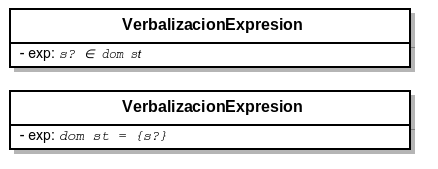
\includegraphics[scale=0.4]{img/mensajes.png}
	\caption{Mensajes a comunicar para el ejemplo de la figura~\ref{fig:ej_test_desc}.}
  	\label{fig:ej_mensajes}
\end{figure}

Vale la pena aclarar que en nuestro caso, los datos con los que trabajamos resultan esquemas Z de las clases de prueba, por lo que ya se encuentran modelados de antemano y no es necesario realizar un nuevo modelo del dominio.
 

\section{Determinación del contenido}
\label{cap:determinacion_contenido}

Como mencionamos anteriormente, en la \emph{determinación de contenido} se suelen llevar a cabo una o más tareas de \emph{selección}, \emph{resumen} y \emph{razonamiento con los datos}. En la figura \ref{fig:tareas_determinacion_contenido} podemos observar el orden en que realizaremos estas tareas y a continuación estudiaremos cada una de ellas detalladamente.

\begin{figure}[H]
  	\centering
	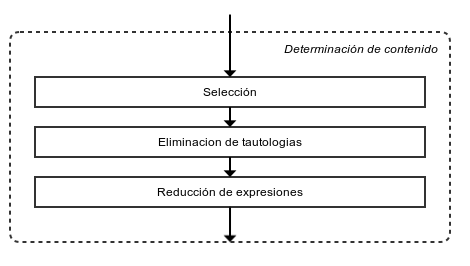
\includegraphics[scale=0.4]{img/tareas_determinacion_contenido.png}
	\caption{Tareas determinación de contenido.}
  	\label{fig:tareas_determinacion_contenido}
\end{figure}

\subsection*{Selección}
Como vimos en la sección anterior, nuestro sistema de NLG deberá ser capaz de producir descripciones para un subconjunto de clases de prueba del total de las clases generadas por \emph{Fastest} para una especificación. Es decir, el usuario podría solicitarle a nuestro sistema la generación de descripciones para una, un grupo o todas las clases de pruebas generadas y éste debería generar descripciones únicamente para las clases de prueba indicadas. Es por esto que deberemos realizar una \emph{selección de la información} que tendrá que ser incluida dentro del \textit{document plan} a fin de ser comunicada, posteriormente, en el texto final.

Para el caso de nuestro trabajo esta tarea se resumirá a la búsqueda y filtrado de las clases de prueba indicadas por el usuario dentro de todo el conjunto de clases de prueba que forma parte de la entrada del sistema. De forma tal que si, por ejemplo, deseamos generar una descripción para la clase de prueba \emph{LookUp\_SP\_1} del ejemplo anterior, la misión de de esta tarea será la de identificar y seleccionar la clase \emph{LookUp\_SP\_1} entre todas las generadas por \emph{Fastest} que formarán parte de los datos de entrada de nuestro sistema de NLG.
%TODO falta ref despues de \emph{LookUp\_SP\_1}

%TODO agregar grafico aca para ejemplificar?

Ya seleccionadas las clases de prueba con las que debemos trabajar, veremos como podemos mejorar las descripciones de nuestro sistema realizando algunos procesamientos sobre la información seleccionada previo a la construcción del \textit{document plan}. En particular veremos dos tareas que podríamos enmarcar dentro del razonamiento con los datos, la \emph{eliminación de tautologías} y la \emph{reducción de expresiones}. 

\subsection*{Eliminación de tautologías}
Como mencionamos anteriormente, todas las clases de prueba incluidas en el \emph{corpus} fueron generadas utilizando \emph{Fastest 1.6}. Hemos observado que en ciertos casos, esta herramienta genera clases de prueba como la que podemos ver a continuación:

\begin{figure}[H]
  \centering
\begin{schema}{Update\_ SP\_ 2}\\
 st : SYM \pfun VAL \\
 s? : SYM \\
 v? : VAL 
\where
 st = \{ \} \\
 \{ s? \mapsto v? \} \neq \{ \}
\end{schema}
  \caption{Clase de prueba para operación Update\_SP\_2.}
  \label{fig:ej_update_sp_2}
\end{figure}

Podemos observar en este caso, que la siguiente expresión del ejemplo anterior:

\begin{figure}[H]
  \centering
  $\{ s? \mapsto v? \} \neq \{ \}$ 
\end{figure}

\noindent
no aporta información relevante para el usuario, de hecho esta expresión no agrega ninguna restricción para el caso de prueba ya que será siempre verdadera y si intentáramos describir este predicado, terminaríamos con un texto parecido al siguiente:

\begin{figure}[H]
  \centering
  \emph{``el conjunto formado por el par formado por el símbolo a actualizar y el nuevo valor, es distinto al conjunto vacío''}
\end{figure}

\noindent
que además de resultar algo difícil de interpretar, no contribuye al objetivo comunicacional.

Esto nos lleva a concluir, que obtendremos descripciones mas claras si filtramos este tipo de expresiones. En particular, lo deberíamos hacer lo antes posible en el \textit{pipeline} de nuestro sistema y la tarea de determinación de contenido resulta la apropiada para realizar este tipo de procesamiento. De esta forma evitaremos que etapas posteriores, como la de \emph{microplanning} o \emph{realización de superficie} deban ocuparse de la generación de frases que no aportarían mas que confusión al texto final.

En la versión de \emph{Fastest} utilizada en este trabajo solo observamos la aparición de tautologías similares a la del ejemplo anterior con predicados con la siguiente estructura:

\begin{figure}[H]
  \centering
  $\{ a, b, ... , n \} \neq \{ \}$ 
\end{figure}


Por lo tanto, la implementación de nuestro sistema solo necesitará considerar el caso antes mencionado. 

En la figura \ref{fig:ej_elim_tauto} podemos ver ilustrado el comportamiento esperado de la tarea de \emph{eliminación de tautologías} para el ejemplo utilizado anteriormente.

\begin{figure}[H]
  	\centering
	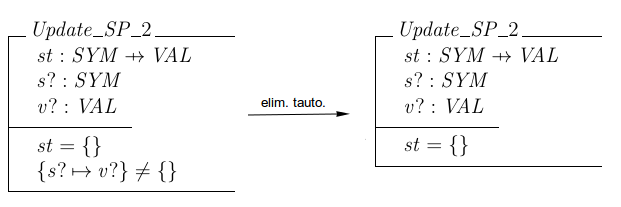
\includegraphics[scale=0.4]{img/ej_elim_tauto.png}
	\caption{Eliminación de tautología para Update\_SP\_2.}
  	\label{fig:ej_elim_tauto}
\end{figure}

Será tarea de nuestro \textit{document planner}, entonces, filtrar tautologías presentes en las clases de prueba para asegurarnos de este modo de que no sean  incluidas dentro del \emph{document plan}.

\subsection*{Reducción de expresiones}
Podemos observar en el \emph{corpus} que hay algunas expresiones que podríamos simplificar y de esta forma lograr descripciones mas claras y concisas. Veamos por ejemplo la figura \ref{fig:ej_update_sp_4}.

\begin{figure}[H]
  \centering
  \begin{schema}{Update\_ SP\_ 4}\\
   st : SYM \pfun VAL \\
   s? : SYM \\
   v? : VAL 
  \where
   st \neq \{ \} \\
   \dom st = \dom \{ s? \mapsto v? \}
  \end{schema}
  \caption{Clase de prueba para operación Update.}
  \label{fig:ej_update_sp_4}
\end{figure}

En particular observemos la expresión:

\begin{figure}[H]
  \centering
  $\dom st = \dom \{ s? \mapsto v? \}$ 
\end{figure}

Si nos adelantamos un poco y tratamos de verbalizar esta expresión de acuerdo a las reglas presentadas en el capítulo \ref{sec:corpus_reglas} podríamos generar una frase como la siguiente:

\begin{figure}[H]
  \centering
  \emph{``el conjunto de símbolos cargados en la tabla es igual a el dominio del par formado por el símbolo a actualiza y el nuevo valor''}
\end{figure}

\noindent
que no parece ser la verbalización mas adecuada para la expresión dada. Por otro lado, veamos que es posible reducir la expresión anterior a la siguiente expresión equivalente:

\begin{figure}[H]
  \centering
  $\dom st = \{s?\}$ 
\end{figure}

\noindent
esta última expresión resultará más fácil de verbalizar, al menos según las reglas introducidas, y se nuestro sistema podría generar una descripción similar a la siguiente:

\begin{figure}[H]
  \emph{``el símbolo a actualizar es el único elemento en la tabla de símbolos cargados''}
\end{figure}

El caso presentado anteriormente fue un caso muy recurrente que que notamos en las clases generadas por \emph{Fastest}. Este resulta de la aplicación de la táctica de partición estándar sobre el operador $\oplus$, lo cual es bastante habitual. Es por esto que creemos importante trabajar este tipo de expresiones antes de incluirlas dentro del \emph{document plan}, para esto nuestro \emph{document planner} deberá realizar el siguiente remplazo siempre que sea posible:

\begin{figure}[H]
  \centering
  $\dom \{ x \mapsto y \} \rightarrow \{x\}$ 
\end{figure}

En la figura \ref{fig:ej_reduce} podemos ver ilustrado el comportamiento esperado de la tarea de \emph{reducción de expresiones} para el ejemplo utilizado anteriormente.

\begin{figure}[H]
  	\centering
	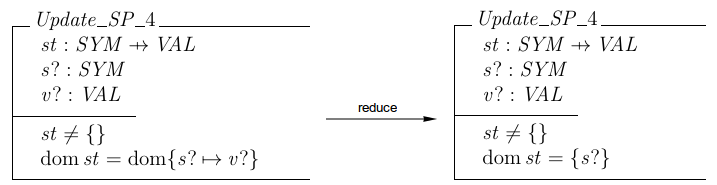
\includegraphics[scale=0.4]{img/ej_reduce.png}
	\caption{Eliminación de tautología para Update\_SP\_4.}
  	\label{fig:ej_reduce}
\end{figure}


Será tarea de nuestro \textit{document planner}, entonces, trabajar también este tipo de expresiones antes de construir los mensajes a incluir dentro del \emph{document plan}.

\section{Estructuración del documento}
\label{sec:document_structure}

Como mencionamos anteriormente, el texto generado no podrá ser una colección de frases y palabras al azar. Deberá tener coherencia y poseer una estructura que le permita al lector interpretar con facilidad el contenido del mismo. Para esto, necesitaremos considerar como organizaremos y estructuraremos la información que debemos comunicar a fin de producir un texto razonablemente fácil de leer y comprender.

%~\footnote{Las decisiones sobre como debe estar ordenado y agrupado el documento final son resultado del análisis del \emph{corpus} de descripciones.}
Esta tarea se concentrará en construir una estructura que contenga la información seleccionada y procesada en la etapa de \emph{determinación de contenido}; estableciendo el agrupamiento y ordenamiento de la misma. Esta estructura deberá caracterizar la disposición de los elementos pertenecientes a los textos recopilados en el \emph{corpus}. De este, podemos observar que los documentos a generar poseen una estructura bastante simple y rígida a la vez. Estos están formados por una secuencia de descripciones para las clases de prueba seleccionadas en la etapa de \emph{determinación de contenido}, a su vez, cada una de estas descripciones agrupa los \emph{mensajes} que modelan la verbalización de las expresiones pertenecientes a cada clase, ordenados de la misma forma en la que aparecen en el esquema de la clase de prueba en cuestión. 

Para modelar nuestro \emph{document plan}, utilizaremos un elemento al que llamaremos \emph{DocumentoDP}, este elemento modelará el documento completo (será la raíz de nuestro \emph{document plan}), éste elemento estará contendrá el título para el documento a generar y un conjunto de elementos que modelarán las descripciones de las distintas clases de prueba. Llamaremos \emph{DescripcionClasePrueba} a estos últimos utilizado para modelar las descripciones de las distintas clases de prueba. Estos estarán formado por información general de la clase de prueba a describir (como el nombre de la misma y una pequeña descripción de la operación a testear) y un conjunto de los \emph{mensajes} introducidos anteriormente: \emph{VerbalizacionExpresion} que modelaran las verbalizaciones de las expresiones Z contenidas dentro de las clases de prueba. En la figura~\ref{fig:png_document_plan} podemos observar una representación abstracta de la estructura que tendrá nuestro \emph{document plan}.

\begin{figure}[H]
  	\centering
	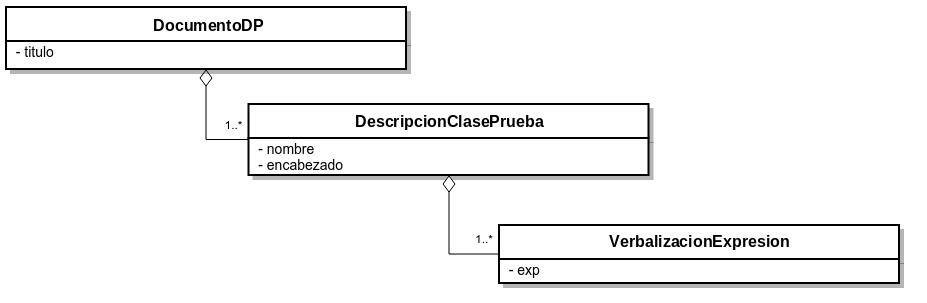
\includegraphics[scale=0.4]{img/document_plan.png}
	\caption{Document plan.}
  	\label{fig:png_document_plan}
\end{figure}

Podemos ver en la figura~\ref{fig:png_document_plan_ej} un ejemplo del document plan para la descripción de la clase de prueba \emph{LookUp\_SP\_1} utilizada en el capítulo anterior (pág \pageref{fig:ej_test_desc}). 

\begin{figure}[H]
  	\centering
	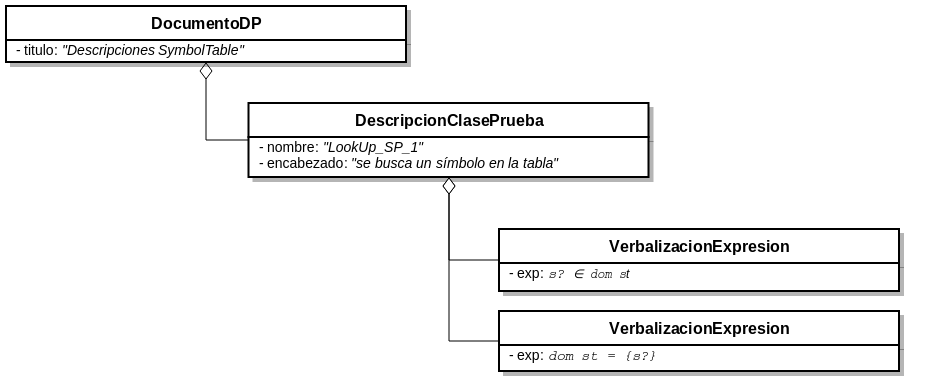
\includegraphics[scale=0.4]{img/document_plan_ej.png}
	\caption{Document plan correspondiente al texto de la figura~\ref{fig:ej_test_desc}.}
  	\label{fig:png_document_plan_ej}
\end{figure}

\bigskip
En este capítulo analizamos las tareas que debe realizar nuestro \emph{document planner}. Como vimos, la misión del mismo es construir un \emph{document plan} que contenga la información requerida por el usuario, filtrada, procesada y agrupada. Tomamos decisiones generales sobre la estructura del documento, dejando para etapas posteriores el trabajo mas detallado, a nivel de las oraciones por ejemplo. Será tarea del \emph{microplanner}, como veremos el próximo capítulo, procesar los \emph{mensajes} construidos en esta etapa y generar a partir de estos una especificación de frase para cada expresión de Z que debemos verbalizar así como también deberá transformar los elementos que contienen información estructural en especificaciones mas concretas del texto a generar (utilizando elementos que modelarán párrafos, secciones, lista de ítems, etc.).
